\chapter{Implementazione}
%‘‘’’
Sia per la realizzazione del front end che del Bootleg Service ho utilizzato TypeScript, sfruttando le funzionalità offerte dalla libreria JavaScript di Radix. 

Per velocizzare lo sviluppo del Bootleg Service, ho usato come base di partenza un server realizzato con TypeScript e WebPack. Ad esso ho aggiunto il codice per la connessione ad un database locale MongoDB, per tenere traccia di tutte le informazioni relative ai bootleg. Essendo a tutti gli effetti un server, per comunicare con il Bootleg Service vengono utilizzate delle normali richieste http, costruite utilizzando la libreria axios.

Per il front end invece ho utilizzato il framework Vue.js, in quanto permette di realizzare un interfaccia utente in maniera piuttosto semplice, e inoltre consente di mantenere le astrazioni di Radix (Atom, Transazioni, ecc.) separate dal codice HTML.

Altri strumenti utili per lo sviluppo del progetto sono stati:
\begin{itemize}
    \item Gli esempi di codice forniti nella documentazione, per mostrare le funzionalità basilari implementabili con la libreria JavaScript: \url{https://docs.radixdlt.com/radixdlt-js/examples/code-examples}.
    \item Applicazione radixdlt-js-showcase, come esempio di frontend Vue.js che utilizza le funzionalità della libreria JavaScript: \url{https://github.com/radixdlt/radixdlt-js-showcase}. 
\end{itemize}

\subsubsection{Scelta dell'Universe}

Come già accennato nel primo capitolo di questa tesi, il concetto di Universe rappresenta la rete Radix. Attualmente sono disponibili diversi Universe di testing ai quali connettersi per testare la propria applicazione (un po' come le reti messe a disposizione di Ethereum per le DApp in fase di sviluppo). La prima cosa che deve fare un'applicazione all'avvio è connettersi con uno di questi Universe a disposizione. Attualmente gli Universe disponibili per la libreria JavaScript sono: BETANET\_EMULATOR, BETANET, LOCALHOST\_SINGLENODE, LOCALHOST e SUNSTONE. In una prima versione dell'applicazione ho deciso di utilizzare l'Universe BETANET\_EMULATOR, in quanto consentiva di avviare l'applicazione senza dover prima avviare il Betanet Emulator sulla propria macchina. 

Solo successivamente ho deciso di aggiungere anche una versione che utilizzasse l'Universe LOCALHOST\_SINGLENODE, che richiede l'avvio del Betanet Emulator per simulare la rete betanet sulla propria macchina. E' possibile avviare l'emulatore attraverso un'immagine Docker, seguendo la procedura spiegata nella documentazione ufficiale di Radix: \url{https://docs.radixdlt.com/kb/develop/betanet-emulator}. 

\section{Utilizzo dei Token}

Per effettuare i pagamenti dei bootleg all'interno dell'applicazione, viene usato il token BTLG. Il Bootleg Service definisce il token BTLG al suo primo avvio come un token multi-issuance. Nel momento in cui un utente crea una nuova identity, il frontend invia una richiesta al Bootleg Service per ricevere una somma iniziale di token BTLG token. In sostanza, il Bootleg Service prende il posto del Faucet, ovvero un account particolare che ha lo scopo di inviare dei token nativi di test. La scelta di creare un token nativo per l'applicazione con il Bootleg Service, e di inviarne una quantità predefinita a ciascuna nuova identity è stata presa soltanto durante l'implementazione del progetto. Inizialmente l'idea era quella di utilizzare il token nativo della piattaforma Radix (denominato XRD) richiedendone l'invio al Faucet Service all'avvio dell'applicazione. Tuttavia, dal momento che l'Universe in Radix influenza la creazione degli indirizzi, in ciascun Universe esiste un Faucet con un indirizzo differente. Non trovando da nessuna parte l'indirizzo del faucet per l'Universe BETANET\_EMULATOR, ho dunque optato per la creazione di un token nativo all'interno dell'applicazione.

Il Bootleg Service ha anche il compito di definire un Token univoco per ciascun bootleg nel momento della sua creazione. Il possesso di questo Token da parte di un utente è ciò che indica al sistema che tale utente ha acquistato il relativo bootleg, e pertanto è autorizzato a visualizzarlo. Inizialmente il bootleg token viene mantenuto dall'account Radix del Bootleg Server, fino a che un utente non decide di acquistare il bootleg.

\section{Gestione dell'identity}

\begin{figure}[H]
    \centering
    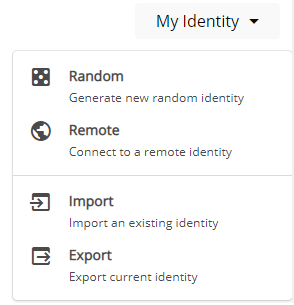
\includegraphics{images/application/identity-manage.png}
    \caption{Funzionalità disponibili per le identity}
    \label{fig:identity_manage}
\end{figure}

La libreria Radix offre delle funzionalità per la gestione delle identity all'interno di un'applicazione. La funzione `encryptKey`, date in input un'identity e una password, cifra la prima producendo in output un oggetto JSON detto anche \textit{keystore}. L'identity viene decifrata usando la funzione `decryptKey`, fornendo in input il keystore e la password utilizzata per produrlo. Per la gestione dell'identity all'interno dell'applicazione sono disponibili due diverse opzioni:
\begin{itemize}
    \item Generare una nuova identity locale.
    \item Usare un'identity remota.
\end{itemize}

\subsubsection{Identity locale}

\begin{figure}[H]
  \centering
  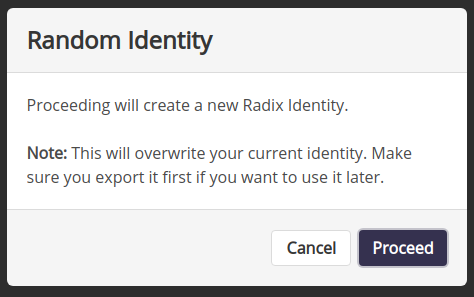
\includegraphics[width=0.75\textwidth]{images/application/create_random.png}
  \caption{Creazione di una nuova identity locale}
  \label{fig:identity_creation}
\end{figure}

Quando l'utente genera una nuova identity locale, questa viene automaticamente cifrata con una password di default e il keystore viene salvato nella memoria del browser utilizzando la proprietà `Window.localStorage`. Quando il frontend viene caricato, controlla la proprietà localStorage, e se è presente un keyStore salvato in precedenza, lo decifra e carica l'identity nell'applicazione. In questo modo, se l'utente chiude e riapre il browser, ritroverà la stessa identity. Quando l'utente genera una nuova identity locale, l'identity presente in localStorage viene sovrascritta e non si può più recuperare. Se l'utente crea un'identity e vuole salvarla per riutilizzarla in un secondo momento, ha la possibilità di \textit{esportare} la propria identity: Facendo con la funzione ‘‘Export’’ l'applicazione chiede all'utente di inserire una password per cifrare la chiave, e una volta scelta la password, mostra all'utente il keystore JSON prodotto. 

\begin{figure}[H]
    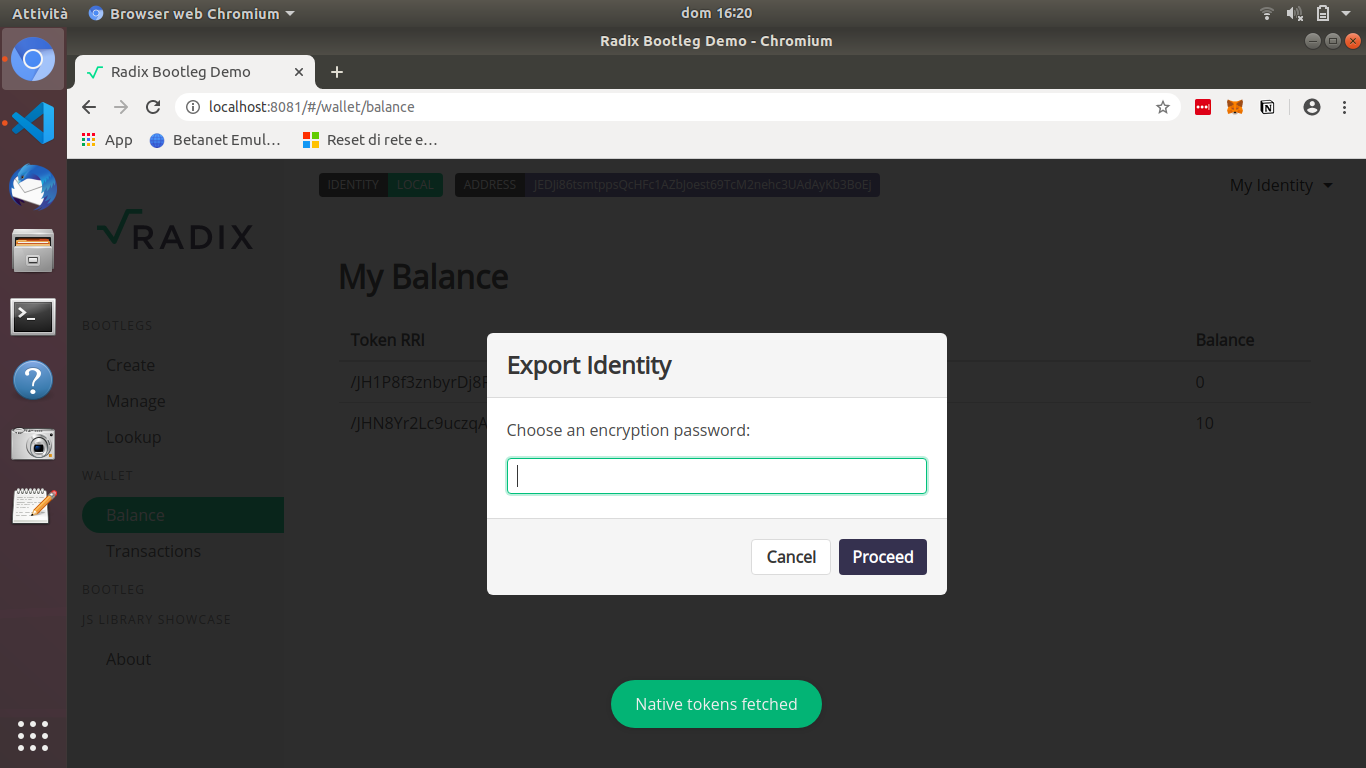
\includegraphics[width=\linewidth]{images/application/choose-password.png}
    \caption{Scelta della password per la creazione del keystore}
    \label{fig:choose_password}
\end{figure}

L'utente può così copiare il contenuto del keystore e salvarlo all'interno di un file, in modo da poterlo recuperare in un secondo momento. L'utente può successivamente importare l'identity creata in precedenza con la funzione \textit{import}: L'utente inserisce il keystore e la password associata per decriptare il keystore, e così facendo l'identity viene importata nell'applicazione.

\begin{figure}[H]
  \centering
  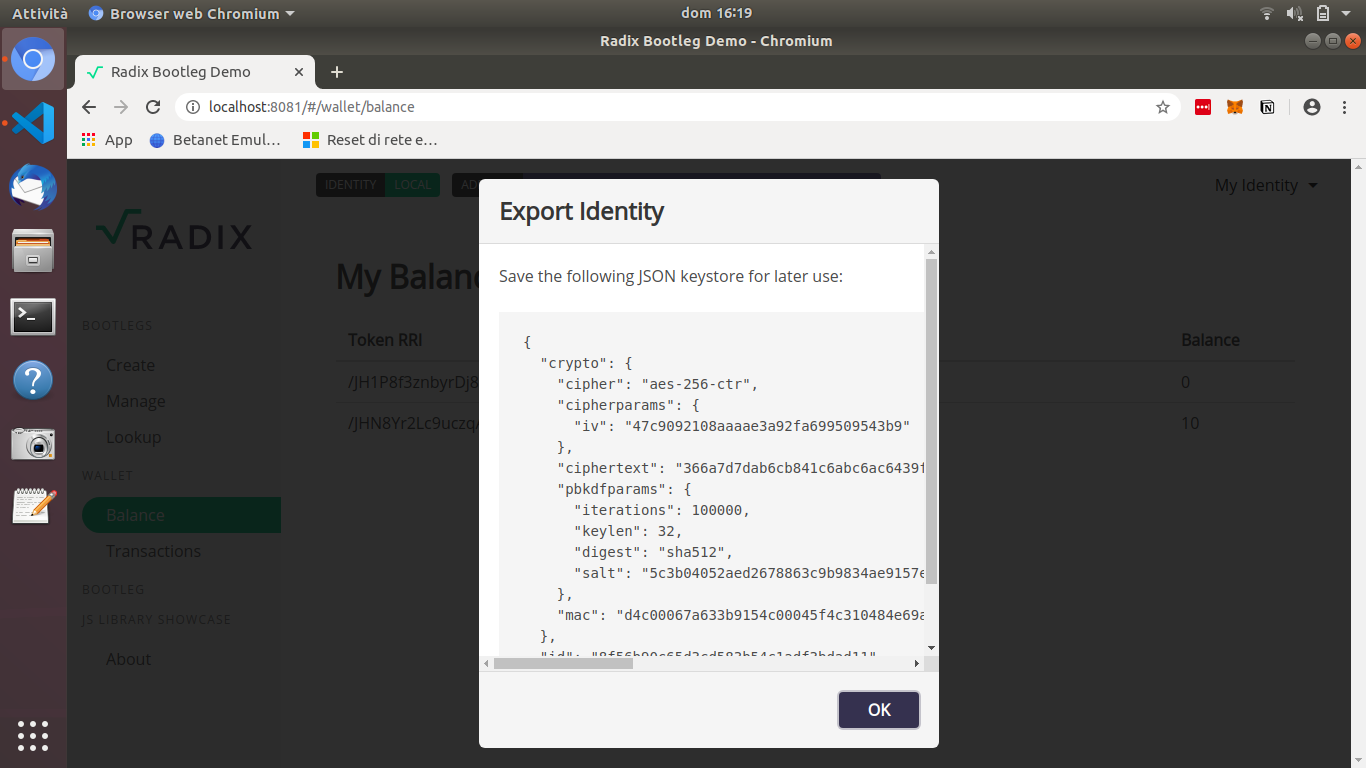
\includegraphics[scale=0.4]{images/application/save-keystore.png}
  \caption{Visualizzazione del keystore prodotto durante sportazione di un'identity locale}
  \label{fig:save_keystore}
\end{figure}

\subsubsection{Identity remota}

Usando un'identity remota invece, l'applicazione userà la chiave privata salvata nel Radix Wallet dell'utente, che pertanto non necessita di essere salvata nel browser. In questo caso, l'applicazione invia una richiesta al Radix Wallet. Una volta che l'utente accetta la richiesta, l'applicazione potrà usare la chiave privata mantenuta nel Wallet per firmare atom per conto dell'utente.
Mentre il Frontend consente la gestione di un'identity per conto dell'utente, il Bootleg Service ha una propria identity, che viene creata al suo primo avvio, e ripristinata agli avvii successivi. Anche in questo caso vengono utilizzate le funzioni encryptKey e decryptKey, combinate con la scrittura del keystore su un file .json. Al suo avvio, il Bootleg Service cerca il file contenente il keystore, e se lo trova, ne decifra il contenuto e carica l'identity, altrimenti ne crea una nuova.

\section{Creazione di un bootleg}

Per creare un bootleg, è necessario inserire:
\begin{itemize}
    \item Simbolo usato per il token;
    \item Titolo del bootleg;
    \item Indirizzo dell'artista;
    \item Prezzo del bootleg;
    \item Url del bootleg (Per semplicità sono stati utilizzati dei link di video su YouTube);
\end{itemize}

\begin{figure}[H]
    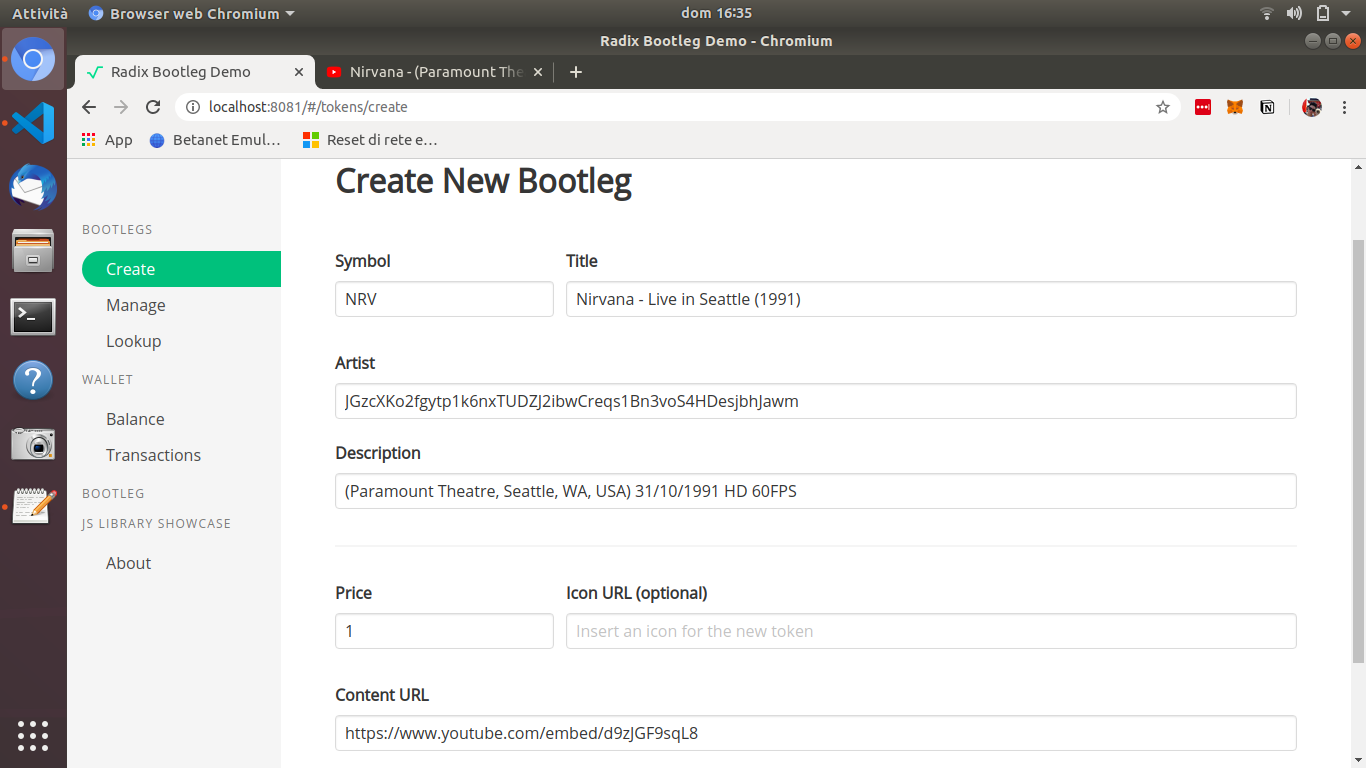
\includegraphics[width=\linewidth]{images/application/create-bootleg.png}
    \caption{Creazione del bootleg}
    \label{fig:bootleg_create}
\end{figure}

Quando l'utente da la conferma, questi vengono inviati al server (Bootleg Service), che provvederà a creare il token per il bootleg e salverà tutti i dati inviati dall'utente sul database, insieme all'identificativo del token appena creato, ed agli indirizzi di bootlegger e artista. Terminato l'inserimento, il Bootleg Service invierà all'utente l'identificativo del token come conferma.

\section{Acquisto di un bootleg}

L'applicazione recupera la lista dei bootleg inseriti sul database inviando una richiesta al Bootleg Service, che esegue una query e recupera tutti i dati dei bootleg (ad eccezione dell'url del video), e li invia al frontend.

Per ciascun bootleg nella lista, il front end verifica se sono presenti nell'account dell'utente, e in caso contrario mostra un pulsante ‘‘Buy’’.

\begin{figure}[H]
    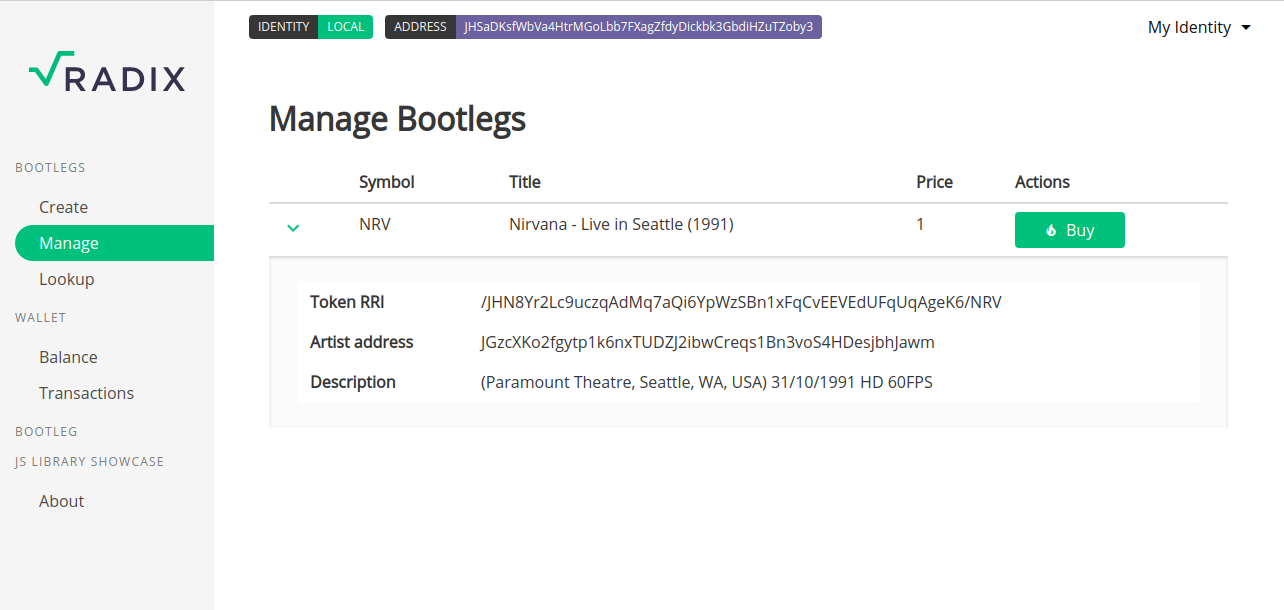
\includegraphics[width=\linewidth]{images/application/manage-bootleg2.png}
    \caption{Finestra di gestione dei bootleg}
    \label{fig:manage_bootleg}
\end{figure}

Quando un utente acquista un bootleg, l'applicazione verifica che il suo account possieda un ammontare sufficiente di BTLG. Se si, il pagamento viene inviato al Bootleg Service, insieme ai dati del bootleg da acquistare. Il Bootleg Service può così dividere il pagamento in parti uguali tra artista, bootlegger ed eventuali franchisor.

Una volta che il pagamento è stato diviso tra i vari destinatari, il Bootleg Service procede con l'invio del token all'utente ed inserisce quest'ultimo nella lista dei franchisor per quel token, aggiornando i dati sul database. In questo modo, quando verrà effettuato un nuovo acquisto del bootleg, l'utente riceverà una percentuale del pagamento come franchisor. 

\section{Visualizzazione del bootleg}

Una volta che l'utente possiede il token, nella lista dei bootleg compare il pulsante ‘‘Watch’’ di fianco al bootleg, che consente all'utente di visualizzare il bootleg. Dal momento che il front-end non possiede di per se l'url del video, deve richiederlo al Bootleg Service. Il modo in cui il frontend richiede ed ottiene il link al contenuto del bootleg si basa su uno schema challenge-response. 

\begin{figure}[H]
    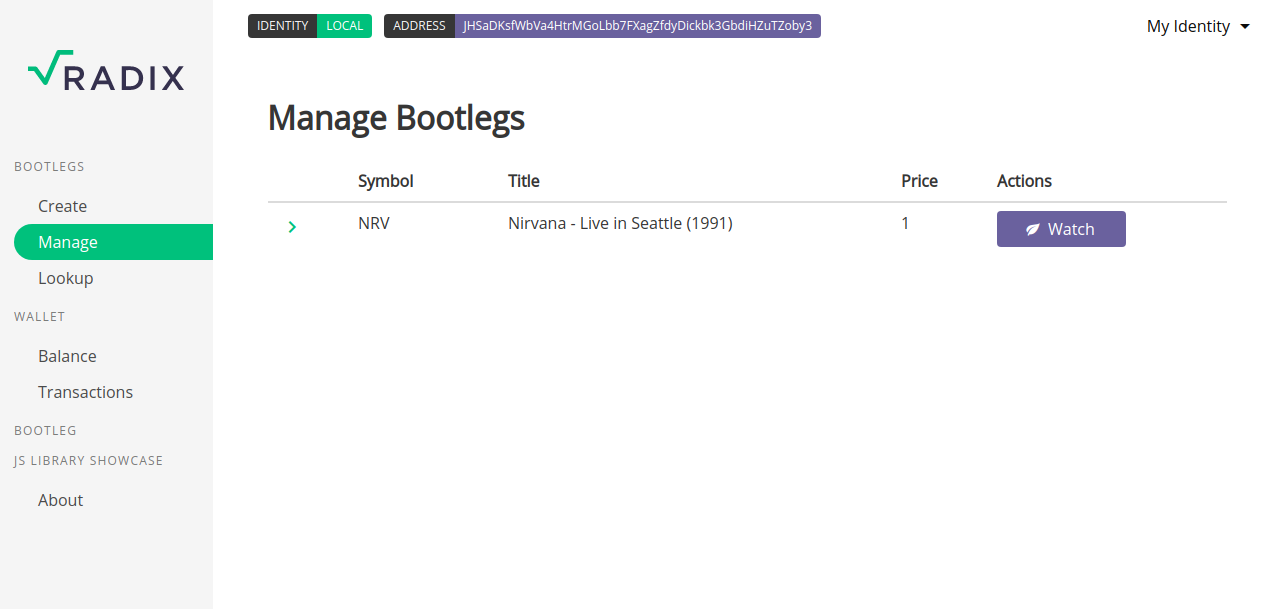
\includegraphics[width=\linewidth]{images/application/bootleg-purchased.png}
    \caption{Bootleg acquistato}
    \label{fig:bootleg_purchased}
\end{figure}

Cliccando su ‘‘Watch’’ il front end invia una richiesta al Bootleg Service per il link al bootleg.Quando il DS riceve questa richiesta, genera una \textit{challenge} casuale, che nel caso specifico dell'applicazione, è un UUID generato con il package uuidv4. La challenge, prima di essere inviata, viene nel database insieme ad un attributo boolean \textit{consumed}, inizialmente settato a ‘‘false’’, per indicare che la challenge non è stata ancora utilizzata per accedere ad un bootleg. 

Quando il frontend riceve la challenge dal Bootleg Service, crea un nuovo Payload Atom, vi inserisce la challenge ottenuta dal Bootleg Service come payload, firma questo Atom con la propria identity e lo invia al Bootleg Service con una richiesta http insieme all'URI del token del bootleg da visualizzare.

Una volta che il Bootleg Service riceve anche questa richiesta:
\begin{enumerate}
    \item Estrae l'atom dalla richiesta e verifica la validità della firma dell'atom, cioè controlla se è stata prodotta dall'account che ha creato l'atom. Se la firma viene verificata con successo, il DS procede con la verifica della challenge.
    \item Verifica la validità della challenge: il DS estrae la challenge dal payload dell'atom, ed esegue una query sul database per trovare la challenge ricevuta. Se non viene trovata la challenge, oppure viene trovata ma l'attributo ‘‘consumed’’ ha valore ‘‘true’’ (dunque è già stata utilizzata), la challenge non viene considerata valida e il DS restituisce un errore al frontend. Altrimenti, aggiorna il valore di ‘‘consumed’’ a true sul database e prosegue al passo successivo.
    \item Verifica il possesso del bootleg: Il DS controlla il saldo dell'account dell'utente che ha inviato la richiesta e verifica se è presente il token del bootleg richiesto. Se il token è presente, allora il DS recupera il link del video dal database e lo invia come risposta al frontend.
\end{enumerate}

Una volta che il frontend riceve il link del bootleg, mostra all'utente il video YouTube attraverso un elemento `<iframe>`.
\begin{figure}[H]
    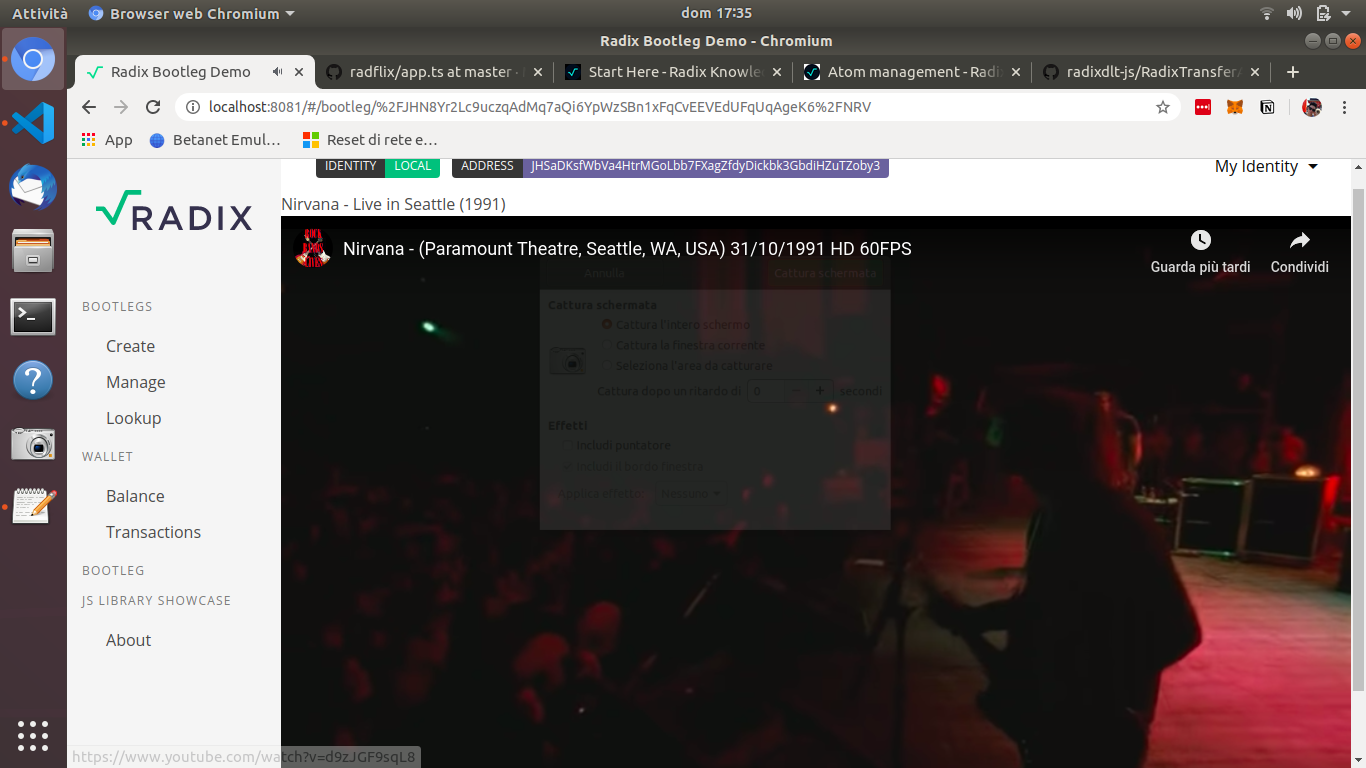
\includegraphics[width=\linewidth]{images/application/watch.png}
    \caption{Visualizzazione del bootleg}
    \label{fig:watch}
\end{figure}

\section{Visualizzazione del saldo e delle transazioni}

L'applicazione consente inoltre all'utente di visualizzare le transazioni ricevute e inviate, nonché il saldo dei token presenti sul proprio account.

\begin{figure}[H]
    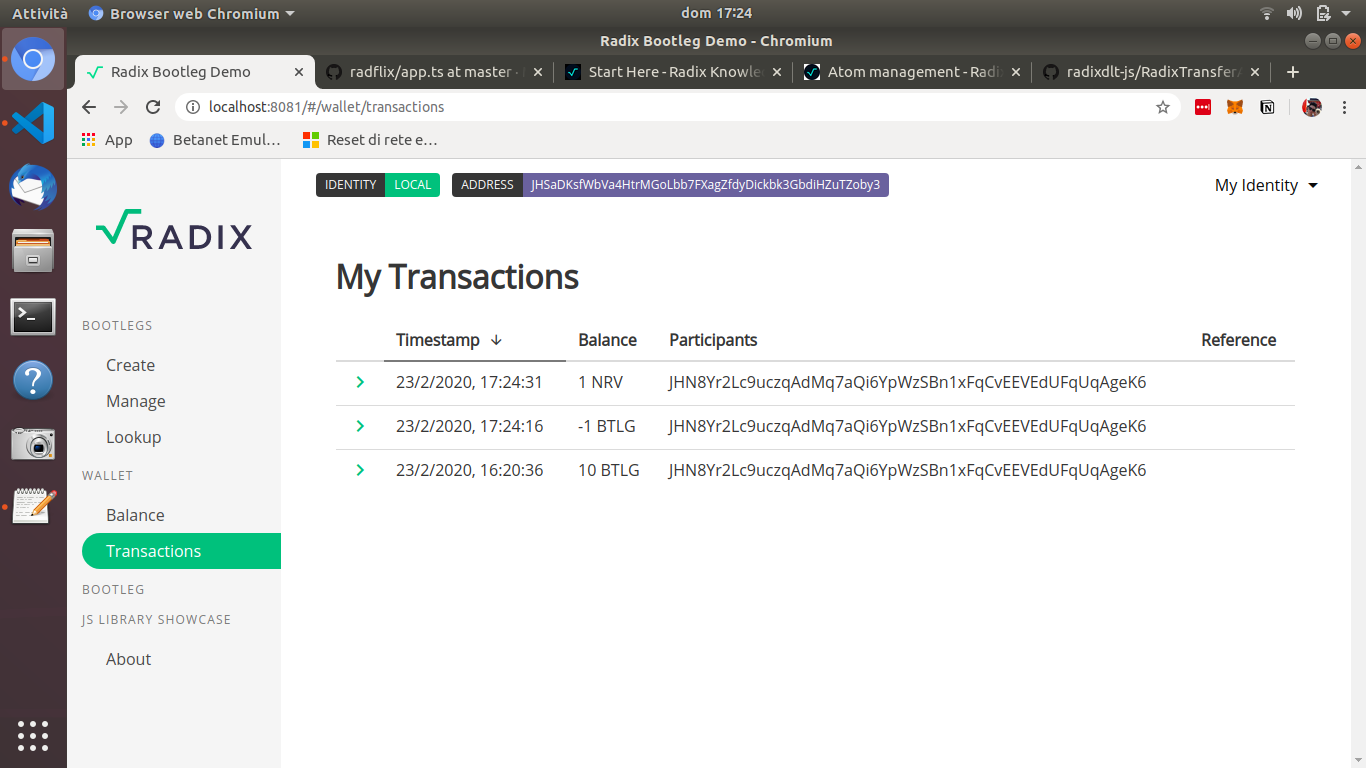
\includegraphics[width=\linewidth]{images/application/transactions.png}
    \caption{Visualizzazione delle transazioni che coinvolgono l'account}
    \label{fig:transactions}
\end{figure}

\begin{figure}[H]
    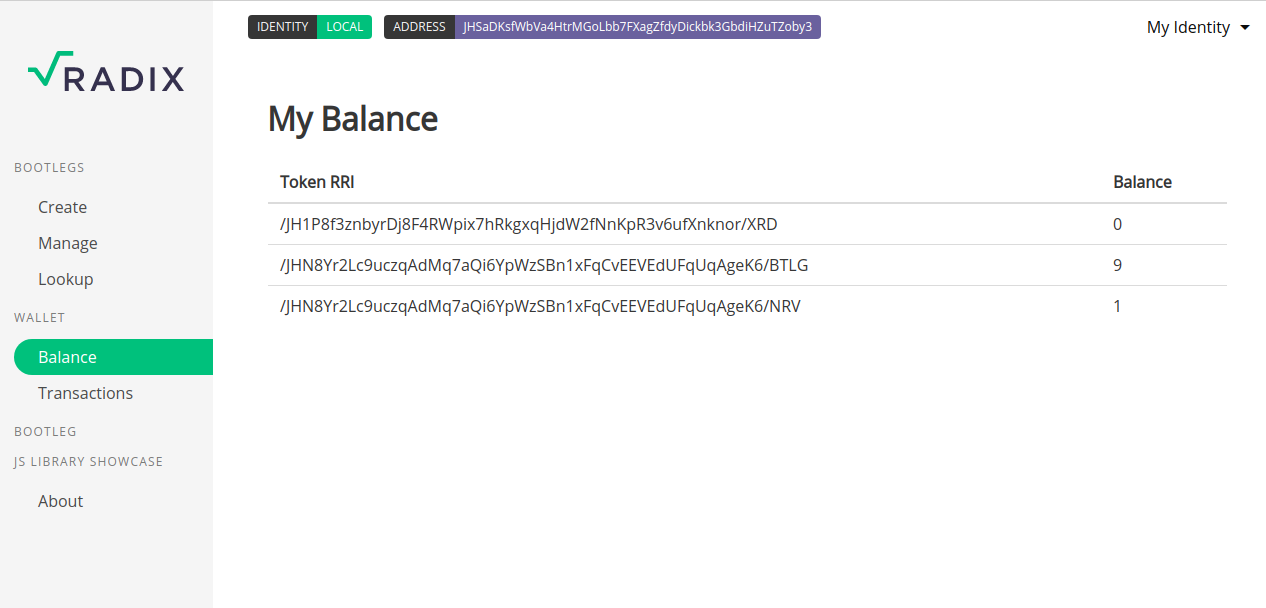
\includegraphics[width=\linewidth]{images/application/balance.png}
    \caption{Visualizzazione del saldo dell'account}
    \label{fig:balance}
\end{figure}